% This LaTeX was auto-generated from MATLAB code.
% To make changes, update the MATLAB code and export to LaTeX again.

\documentclass{article}

\usepackage[utf8]{inputenc}
\usepackage[T1]{fontenc}
\usepackage{lmodern}
\usepackage{graphicx}
\usepackage{color}
\usepackage{listings}
\usepackage{hyperref}
\usepackage{amsmath}
\usepackage{amsfonts}
\usepackage{epstopdf}
\usepackage{matlab}

\sloppy
\epstopdfsetup{outdir=./}
\graphicspath{ {./ELEC300F2016Sols_images/} }

\begin{document}

\matlabtitle{ELEC 300 Spring 2018}

\begin{par}
\begin{flushleft}
15.7 Nillison
\end{flushleft}
\end{par}

\begin{par}
\begin{flushleft}
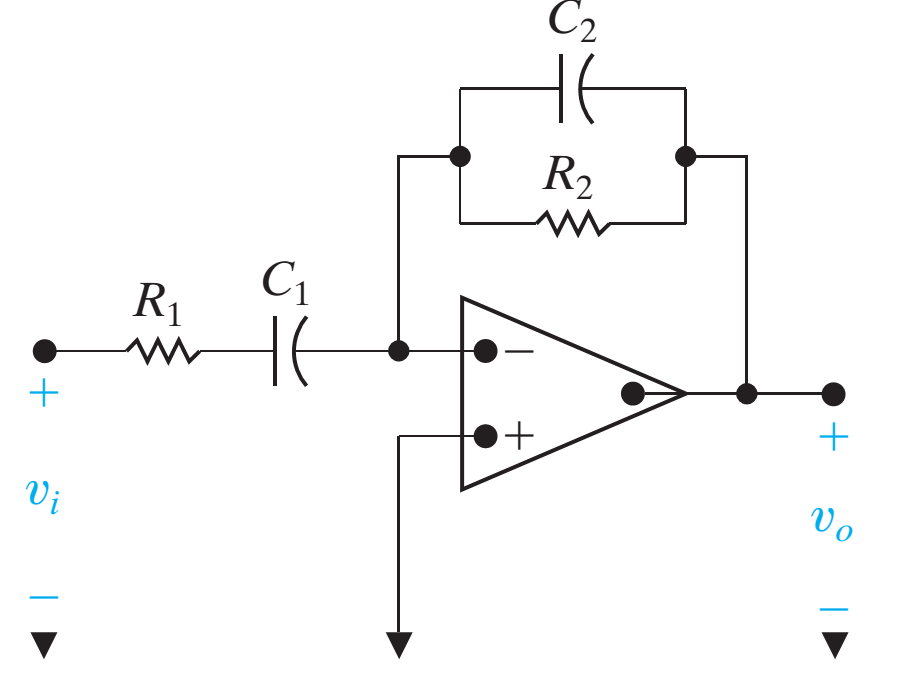
\includegraphics[width=\maxwidth{91.21926743602609em}]{image_0}
\end{flushleft}
\end{par}

\begin{par}
\begin{flushleft}
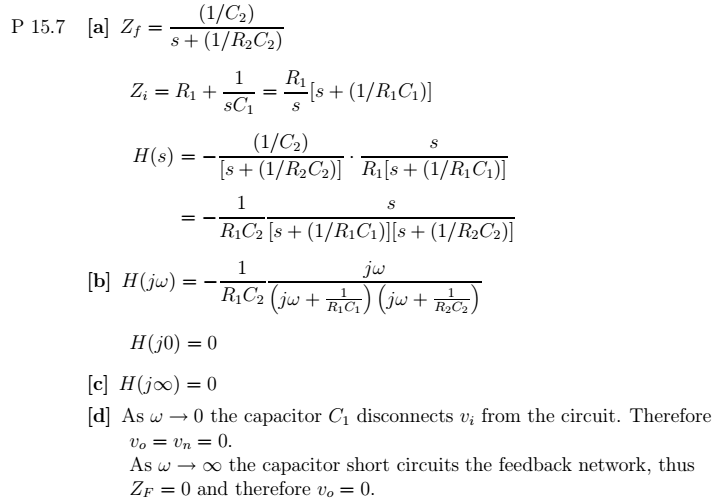
\includegraphics[width=\maxwidth{71.75112895132966em}]{image_1}
\end{flushleft}
\end{par}


\vspace{1em}


\begin{par}
\begin{flushleft}
Sketch the bode plot of $H(s)=\frac{10}{s(s^2+s+16)}$
\end{flushleft}
\end{par}

\begin{matlabcode}
Q2H = tf([10],[1 1 16 0])
\end{matlabcode}
\begin{matlaboutput}
Q2H =
 
         10
  ----------------
  s^3 + s^2 + 16 s
 
Continuous-time transfer function.
\end{matlaboutput}
\begin{matlabcode}
BodePlotGui(Q2H)
\end{matlabcode}

\begin{par}
\begin{flushleft}
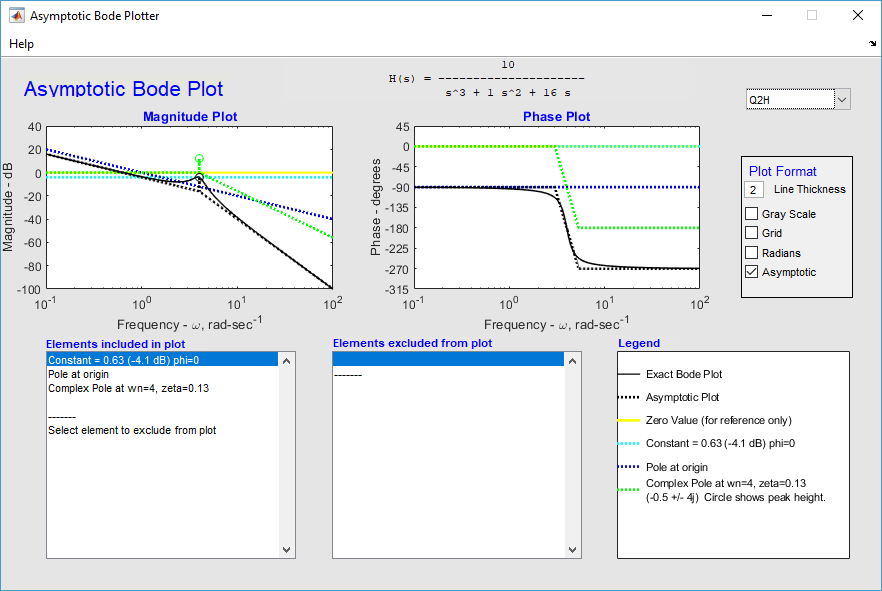
\includegraphics[width=\maxwidth{88.509784244857em}]{image_2}
\end{flushleft}
\end{par}


\begin{par}
\begin{flushleft}
The approximation is pretty good.
\end{flushleft}
\end{par}

\begin{matlabcode}
figure
bode(Q2H)
\end{matlabcode}
\begin{center}
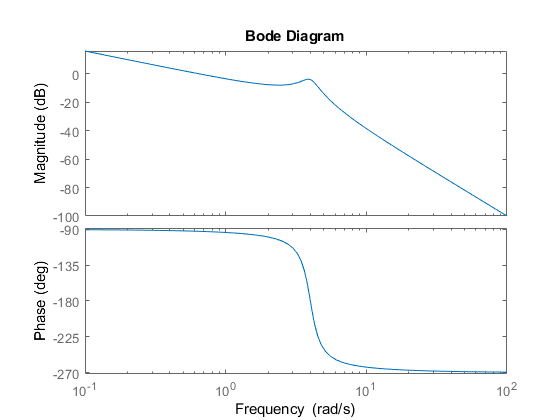
\includegraphics[width=\maxwidth{56.196688409433015em}]{figure_0}
\end{center}


\begin{par}
\begin{flushleft}
Question 3 (similar to 14.20) Nillison, taken from
\end{flushleft}
\end{par}

\begin{par}
\begin{flushleft}
\textbf{Alexander 6th edition 14.40 }A parallel resonance circuit has a resistance of
\end{flushleft}
\end{par}

\begin{par}
\begin{flushleft}
2 kΩ and half-power frequencies of 86 kHz and
\end{flushleft}
\end{par}

\begin{par}
\begin{flushleft}
90 kHz. Determine:
\end{flushleft}
\end{par}

\begin{par}
\begin{flushleft}
(a) the capacitance
\end{flushleft}
\end{par}

\begin{par}
\begin{flushleft}
(b) the inductance
\end{flushleft}
\end{par}

\begin{par}
\begin{flushleft}
(c) the resonant frequency
\end{flushleft}
\end{par}

\begin{par}
\begin{flushleft}
(d) the bandwidth
\end{flushleft}
\end{par}

\begin{par}
\begin{flushleft}
(e) the quality factor
\end{flushleft}
\end{par}

\begin{matlabcode}
u = symunit
\end{matlabcode}
\begin{matlaboutput}
u = 
  symbolicUnitsCollection with units:

      ampere: [1x1 sym]
      kelvin: [1x1 sym]
    kilogram: [1x1 sym]
       meter: [1x1 sym]
        mole: [1x1 sym]
      second: [1x1 sym]
     candela: [1x1 sym]

  Show all units.

\end{matlaboutput}
\begin{matlabcode}
fc1 = 86*u.kHz
\end{matlabcode}
\begin{matlabsymbolicoutput}
fc1 = 
    $\displaystyle 86 {\textrm{kHz}}$
\end{matlabsymbolicoutput}
\begin{matlabcode}
fc2 = 90*u.kHz
\end{matlabcode}
\begin{matlabsymbolicoutput}
fc2 = 
    $\displaystyle 90 {\textrm{kHz}}$
\end{matlabsymbolicoutput}
\begin{matlabcode}
R   = 2*u.kOhm
\end{matlabcode}
\begin{matlabsymbolicoutput}
R = 
    $\displaystyle 2 {\textrm{kΩ}}$
\end{matlabsymbolicoutput}
\begin{matlabcode}
% Calculations
wc1 = 2*pi*fc1
\end{matlabcode}
\begin{matlabsymbolicoutput}
wc1 = 
    $\displaystyle 172 \pi  {\textrm{kHz}}$
\end{matlabsymbolicoutput}
\begin{matlabcode}
wc2 = 2*pi*fc2
\end{matlabcode}
\begin{matlabsymbolicoutput}
wc2 = 
    $\displaystyle 180 \pi  {\textrm{kHz}}$
\end{matlabsymbolicoutput}
\begin{matlabcode}
B = wc2 - wc1
\end{matlabcode}
\begin{matlabsymbolicoutput}
B = 
    $\displaystyle 8 \pi  {\textrm{kHz}}$
\end{matlabsymbolicoutput}
\begin{matlabcode}
w0 = sqrt(wc1*wc2)
\end{matlabcode}
\begin{matlabsymbolicoutput}
w0 = 
    $\displaystyle 12 \pi  \sqrt{215} {\textrm{kHz}}$
\end{matlabsymbolicoutput}
\begin{matlabcode}
Q  = w0 / B
\end{matlabcode}
\begin{matlabsymbolicoutput}
Q = 
    $\displaystyle \frac{3 \sqrt{215}}{2}$
\end{matlabsymbolicoutput}
\begin{matlabcode}
C  = Q/(w0*R)
\end{matlabcode}
\begin{matlabsymbolicoutput}
C = 
    $\displaystyle \frac{1}{16 \pi } \frac{1}{{\textrm{kHz}} {\textrm{kΩ}}}$
\end{matlabsymbolicoutput}
\begin{matlabcode}
Cans  = rewrite(C,u.nF)
\end{matlabcode}
\begin{matlabsymbolicoutput}
Cans = 
    $\displaystyle \frac{125}{2 \pi } {\textrm{nF}}$
\end{matlabsymbolicoutput}
\begin{matlabcode}
L  = 1/(w0^2*C)
\end{matlabcode}
\begin{matlabsymbolicoutput}
L = 
    $\displaystyle \frac{1}{1935 \pi } \frac{{\textrm{kΩ}}}{{\textrm{kHz}}}$
\end{matlabsymbolicoutput}
\begin{matlabcode}
Lans  = rewrite(L,u.H)
\end{matlabcode}
\begin{matlabsymbolicoutput}
Lans = 
    $\displaystyle \frac{1}{1935 \pi } H$
\end{matlabsymbolicoutput}

\begin{par}
\begin{flushleft}
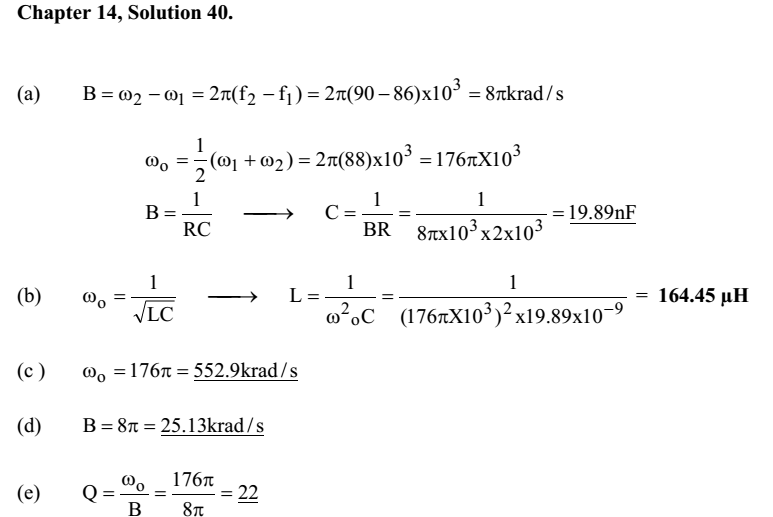
\includegraphics[width=\maxwidth{77.57150025087807em}]{image_3}
\end{flushleft}
\end{par}


\begin{par}
\begin{flushleft}
Design a first-order highpass filter using a non-inverting op amp. The transfer function is given by
\end{flushleft}
\end{par}

\begin{par}
$$H(s)= \frac{1+10^{-3}s}{10^{-3}s}$$
\end{par}

\begin{par}
\begin{flushleft}
Something like the picture below, where Zf = 1/(sC), where C = 100nF, Zi = 10 k Ohm.
\end{flushleft}
\end{par}

\begin{par}
\begin{flushleft}
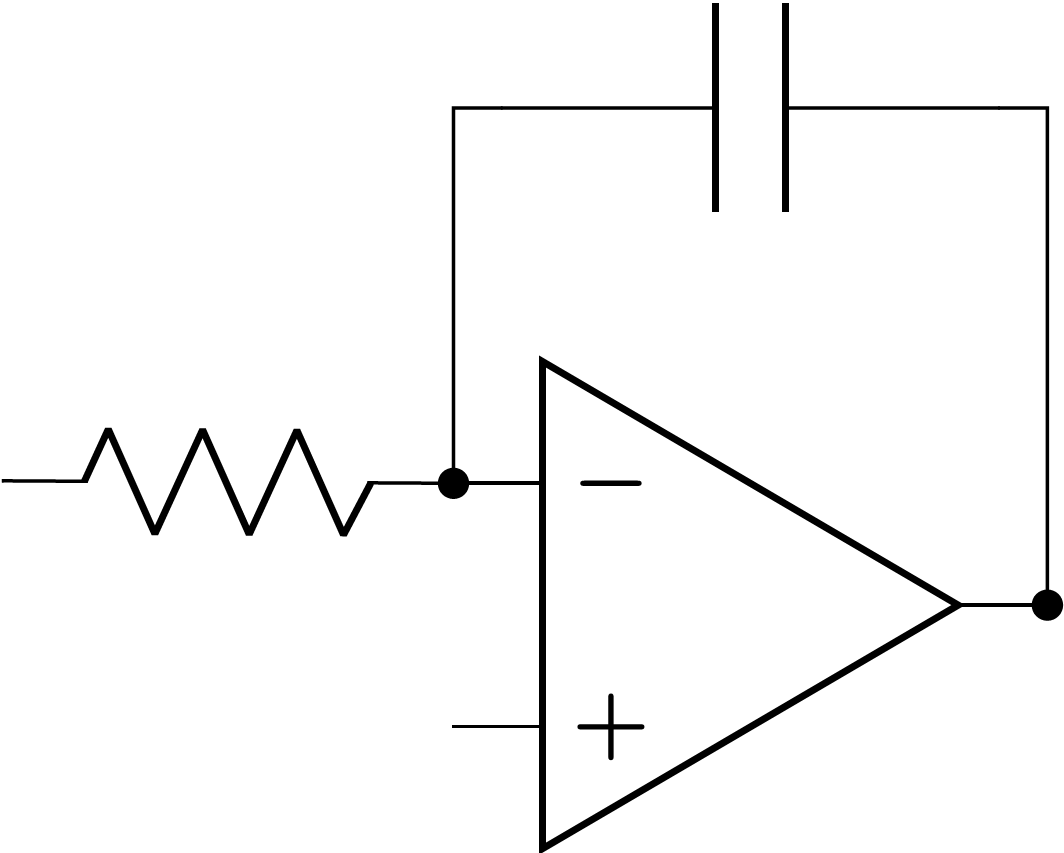
\includegraphics[width=\maxwidth{106.77370797792273em}]{image_4}
\end{flushleft}
\end{par}


\vspace{1em}

\begin{par}
\begin{flushleft}
\textbf{13.45 }For the circuit shown in Fig. 13.110, find the value of the average power absorbed by the 8-Ω
\end{flushleft}
\end{par}

\begin{par}
\begin{flushleft}
resistor.
\end{flushleft}
\end{par}

\begin{par}
\begin{flushleft}
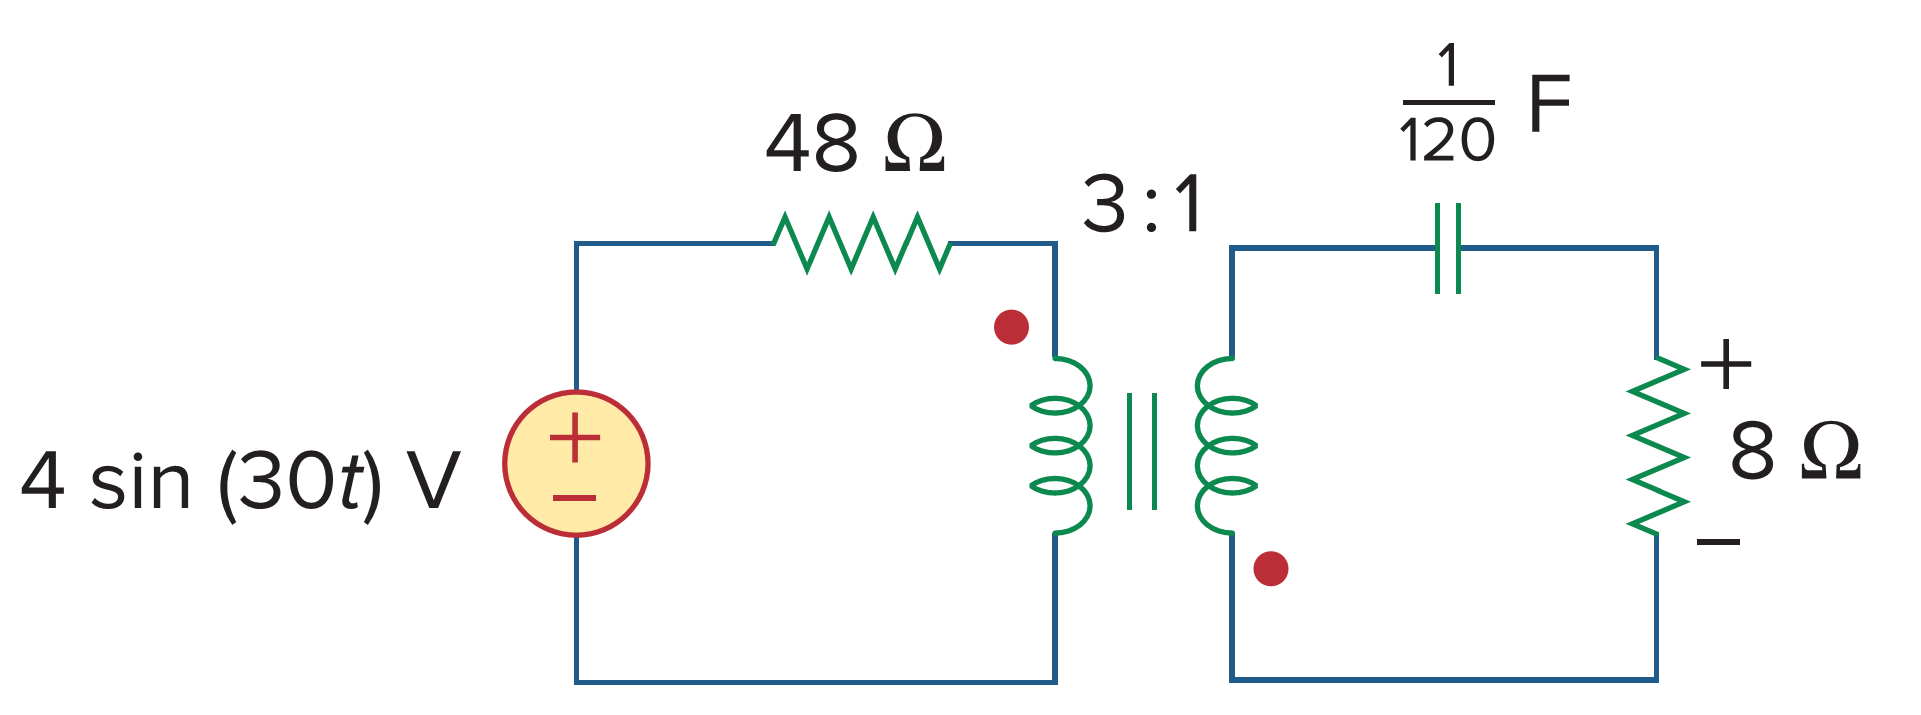
\includegraphics[width=\maxwidth{192.77471149021576em}]{image_5}
\end{flushleft}
\end{par}

\begin{par}
\begin{flushleft}
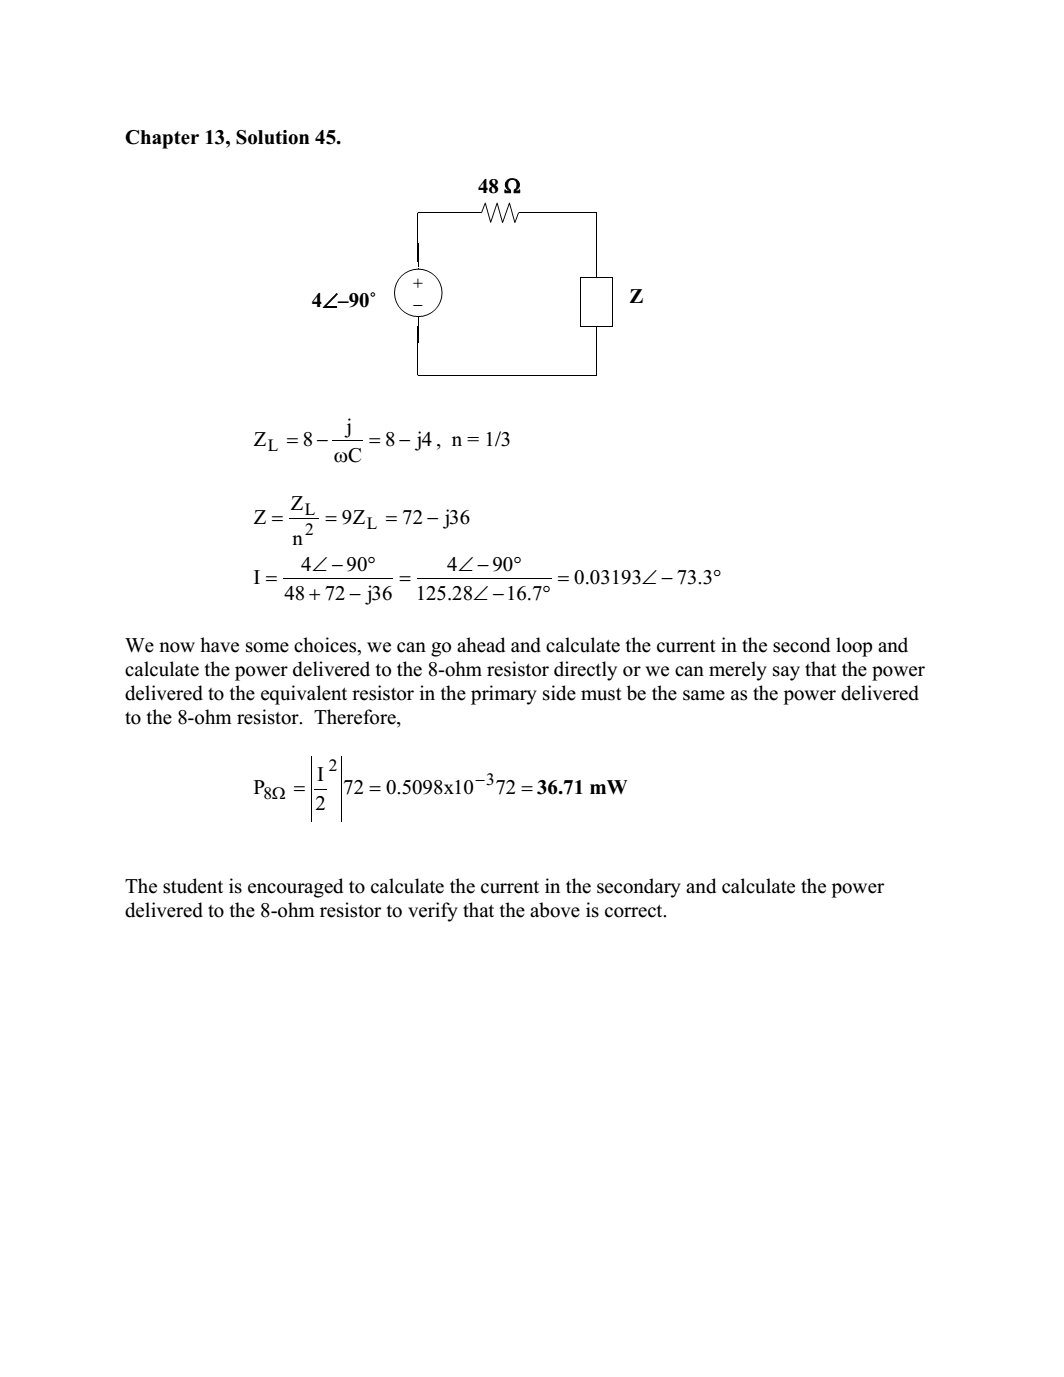
\includegraphics[width=\maxwidth{106.77370797792273em}]{image_6}
\end{flushleft}
\end{par}


\begin{par}
\begin{flushleft}
Question 6) The voltage transfer function of a system is characterized by the following pole-zero plot and a constant of K=100. What is the system's output voltage $v_o(t)$if it is excited by an input voltage of 1 u(t) V?
\end{flushleft}
\end{par}

\begin{matlabcode}
G6s = zpk([0],[-6-j*8 -6+j*8],100)
\end{matlabcode}
\begin{matlaboutput}
G6s =
 
        100 s
  -----------------
  (s^2 + 12s + 100)
 
Continuous-time zero/pole/gain model.
\end{matlaboutput}
\begin{matlabcode}
pzmap(G6s)
\end{matlabcode}
\begin{center}
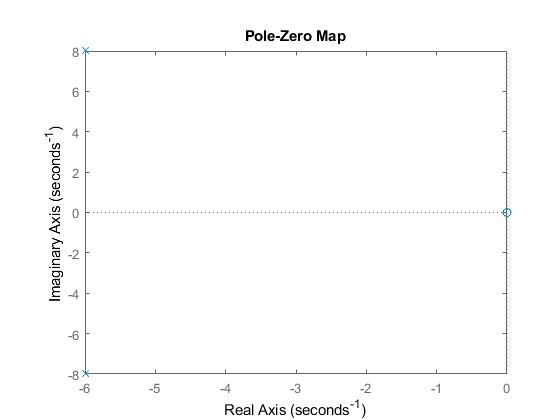
\includegraphics[width=\maxwidth{56.196688409433015em}]{figure_1}
\end{center}


\begin{matlabcode}
syms s
% Found the impulse response
timeFun = ilaplace(s/(s^2+12*s+100))
\end{matlabcode}
\begin{matlabsymbolicoutput}
timeFun = 
    $\displaystyle e^{-6 t}  {\left(\cos \left(8 t\right)-\frac{3 \sin \left(8 t\right)}{4}\right)}$
\end{matlabsymbolicoutput}
\begin{matlabcode}
ezplot(timeFun)
\end{matlabcode}
\begin{center}
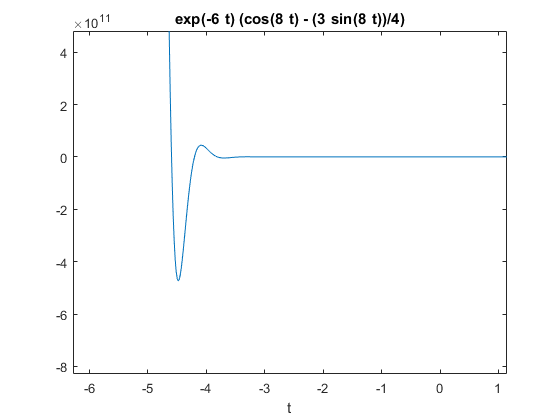
\includegraphics[width=\maxwidth{56.196688409433015em}]{figure_2}
\end{center}
\begin{matlabcode}
% step response 
timeFun2 = ilaplace(1/(s^2+12*s+100))
\end{matlabcode}
\begin{matlabsymbolicoutput}
timeFun2 = 
    $\displaystyle \frac{\sin \left(8 t\right) e^{-6 t} }{8}$
\end{matlabsymbolicoutput}
\begin{matlabcode}
ezplot(timeFun2)
\end{matlabcode}
\begin{center}
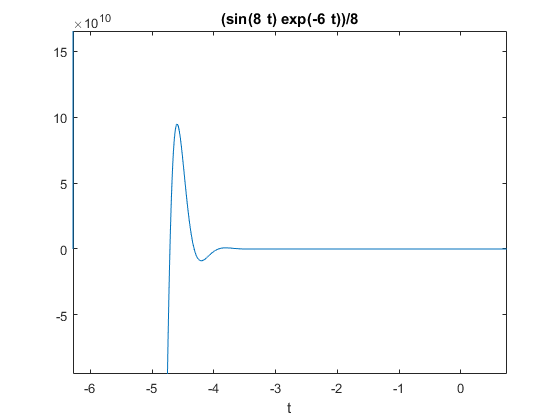
\includegraphics[width=\maxwidth{56.196688409433015em}]{figure_3}
\end{center}
\begin{matlabcode}
step(G6s)
\end{matlabcode}
\begin{center}
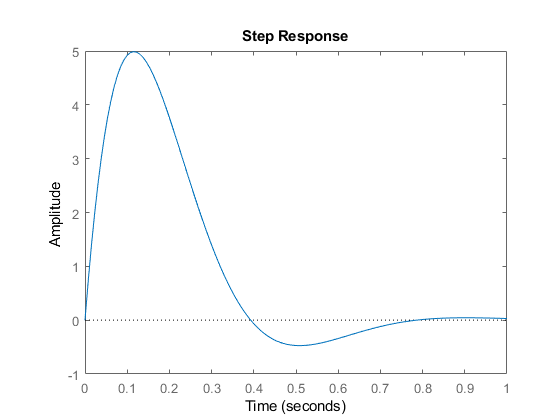
\includegraphics[width=\maxwidth{56.196688409433015em}]{figure_4}
\end{center}


\begin{par}
\begin{flushleft}
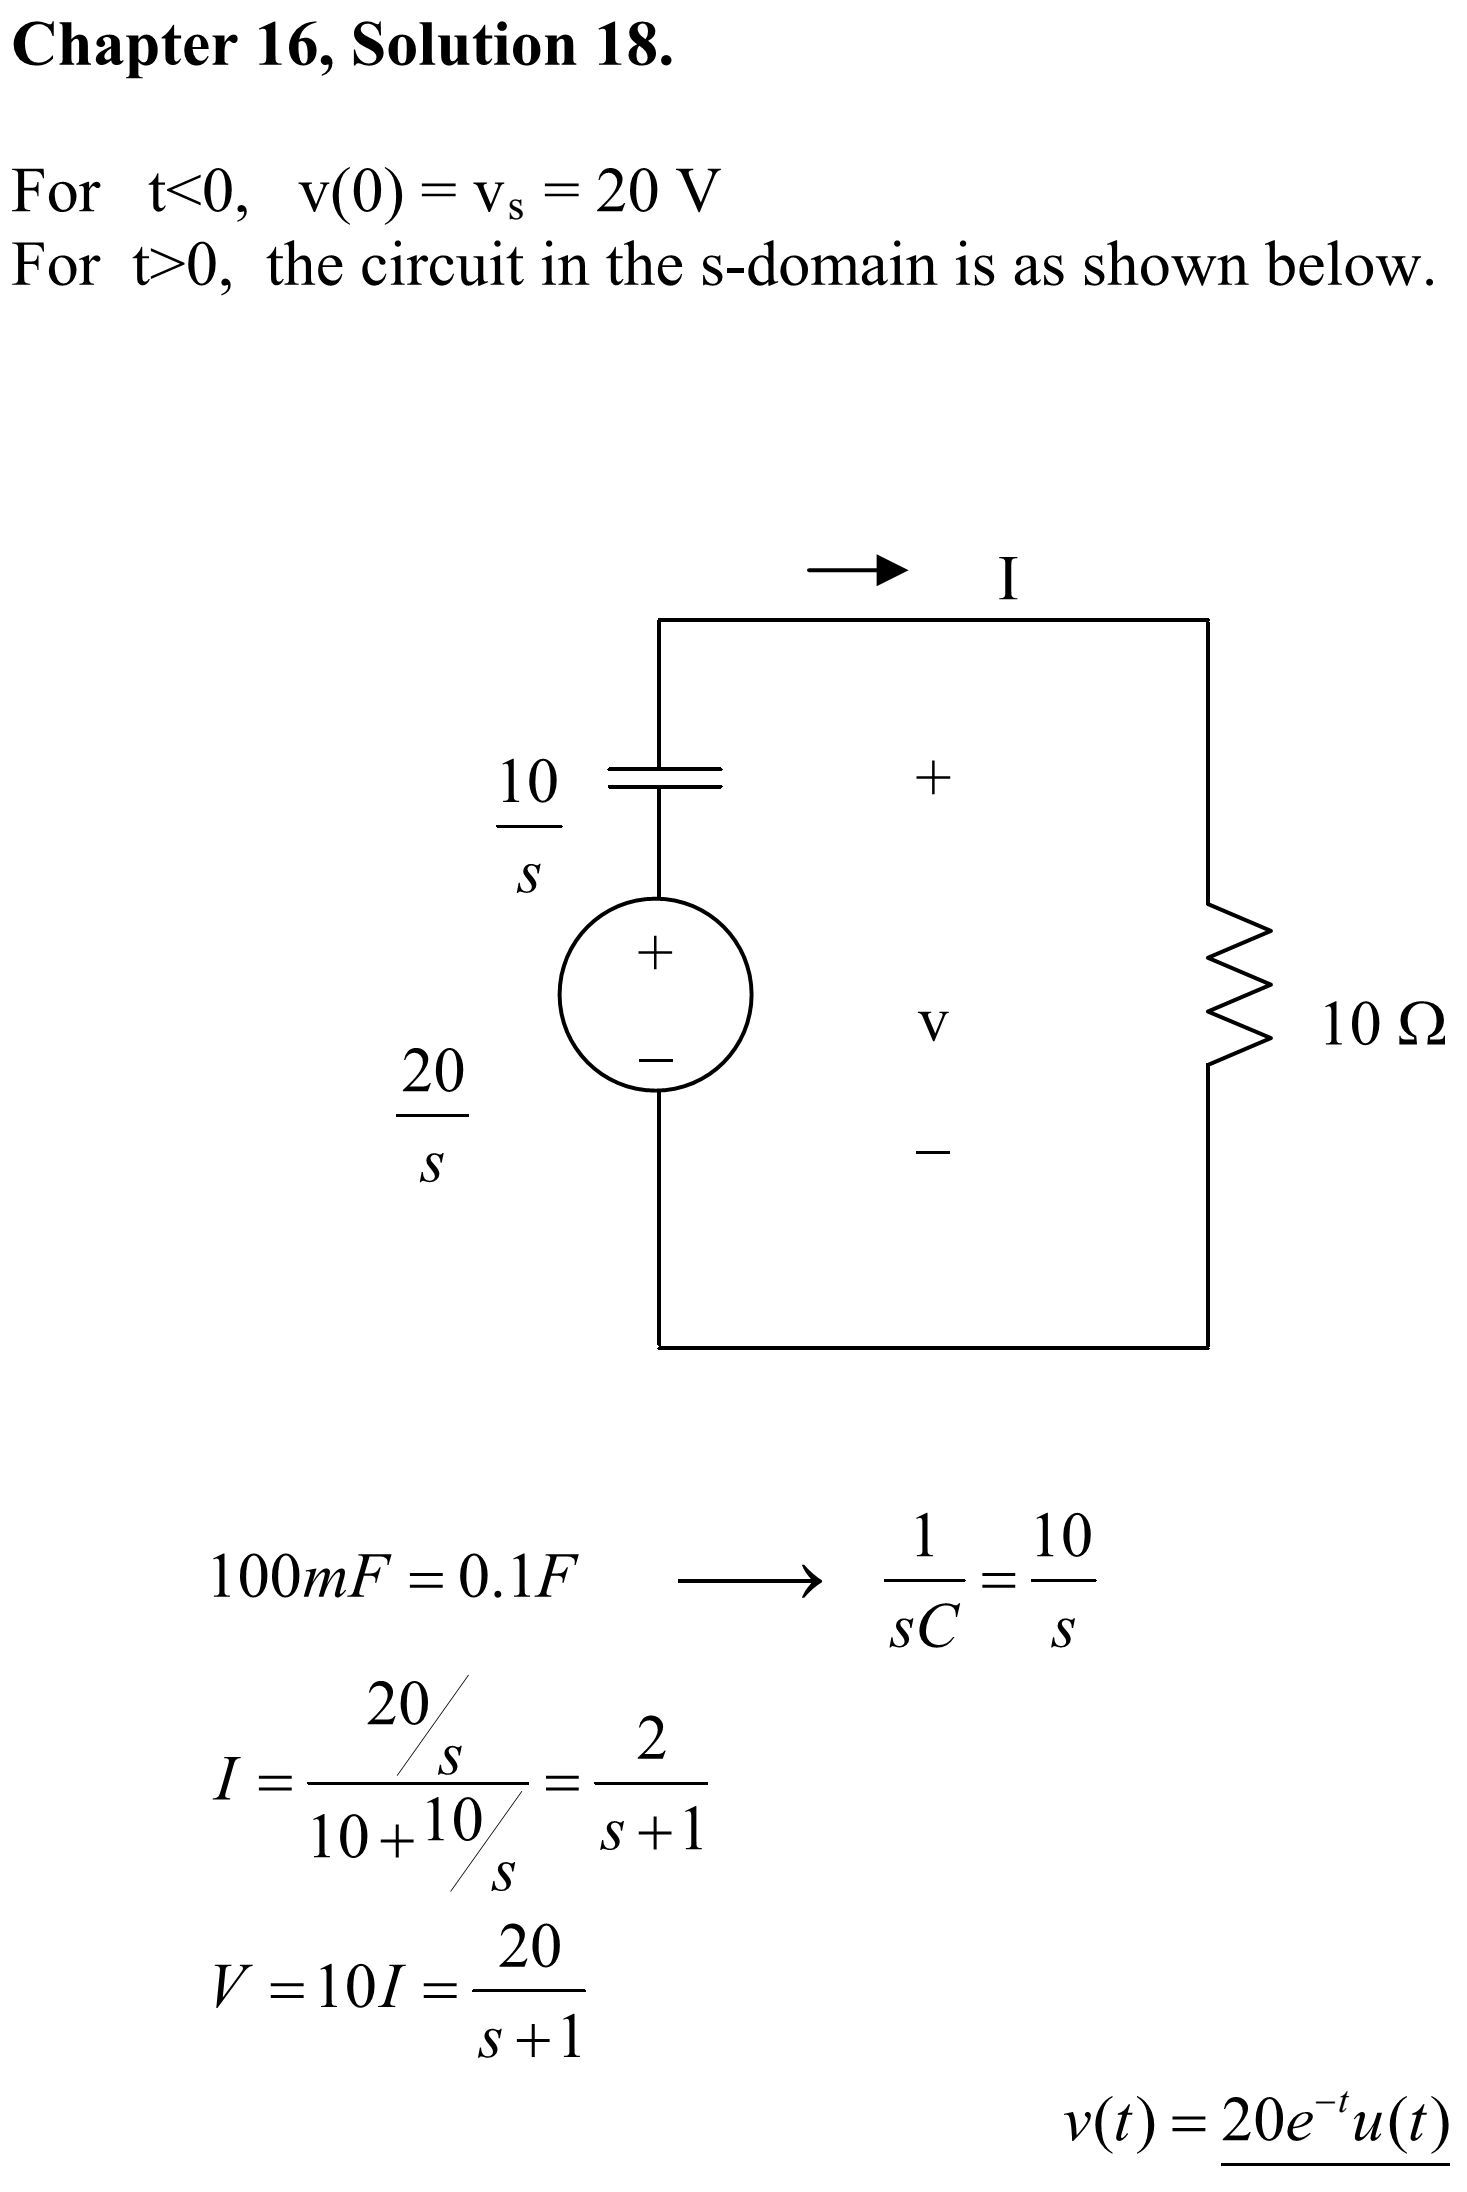
\includegraphics[width=\maxwidth{147.215253386854em}]{image_7}
\end{flushleft}
\end{par}

\vspace{1em}


\begin{par}
\begin{flushleft}
18.19 Nllison
\end{flushleft}
\end{par}

\begin{par}
\begin{flushleft}
    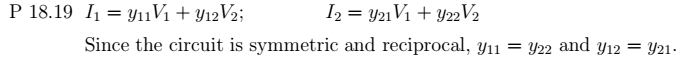
\includegraphics[width=\maxwidth{68.53988961364777em}]{image_8}
\end{flushleft}
\end{par}

\begin{par}
\begin{flushleft}
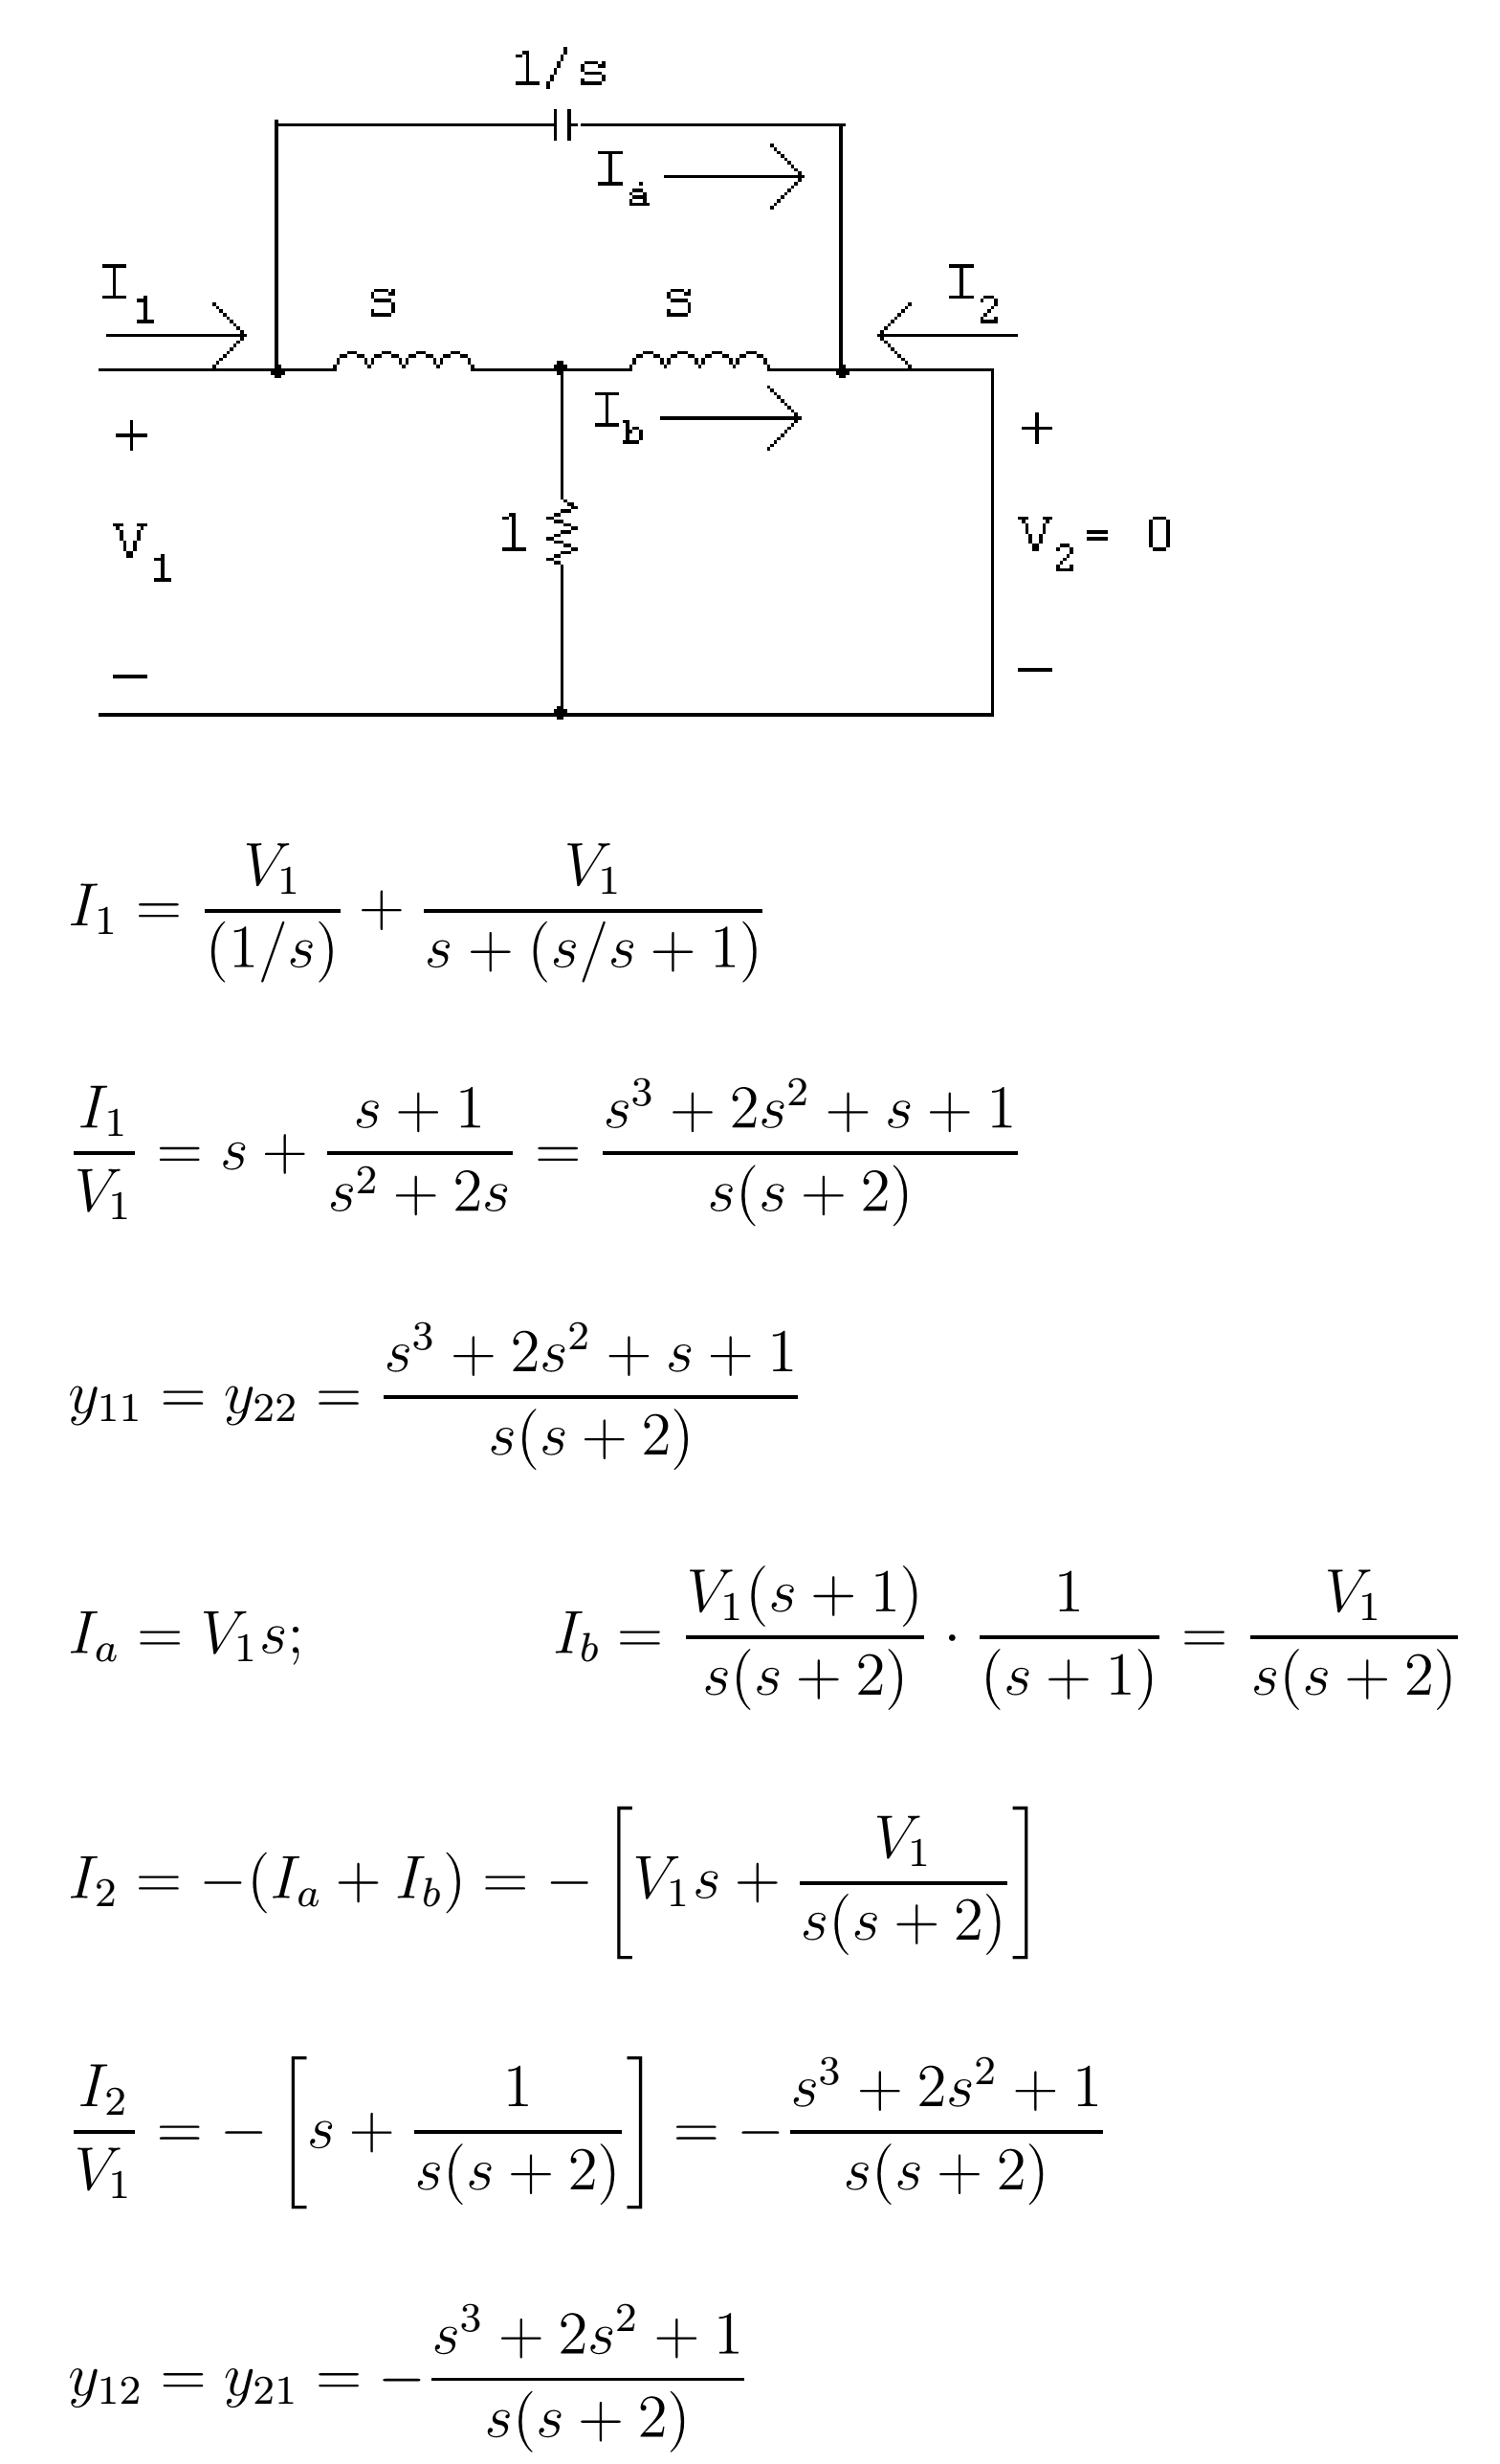
\includegraphics[width=\maxwidth{157.35072754641246em}]{image_9}
\end{flushleft}
\end{par}


\begin{par}
\begin{flushleft}
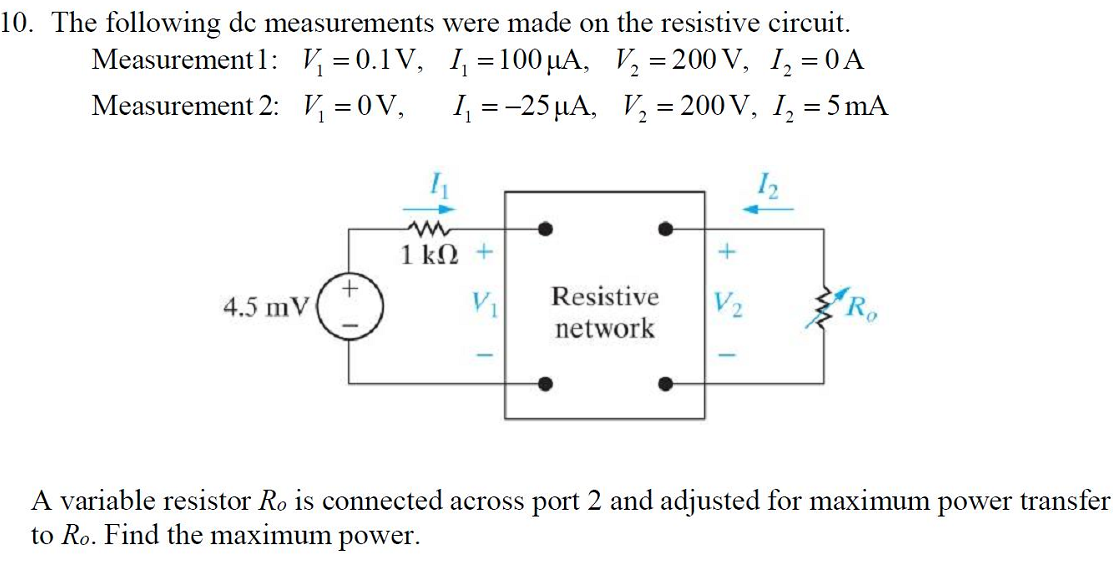
\includegraphics[width=\maxwidth{111.69091821374812em}]{image_10}
\end{flushleft}
\end{par}

\begin{par}
\begin{flushleft}
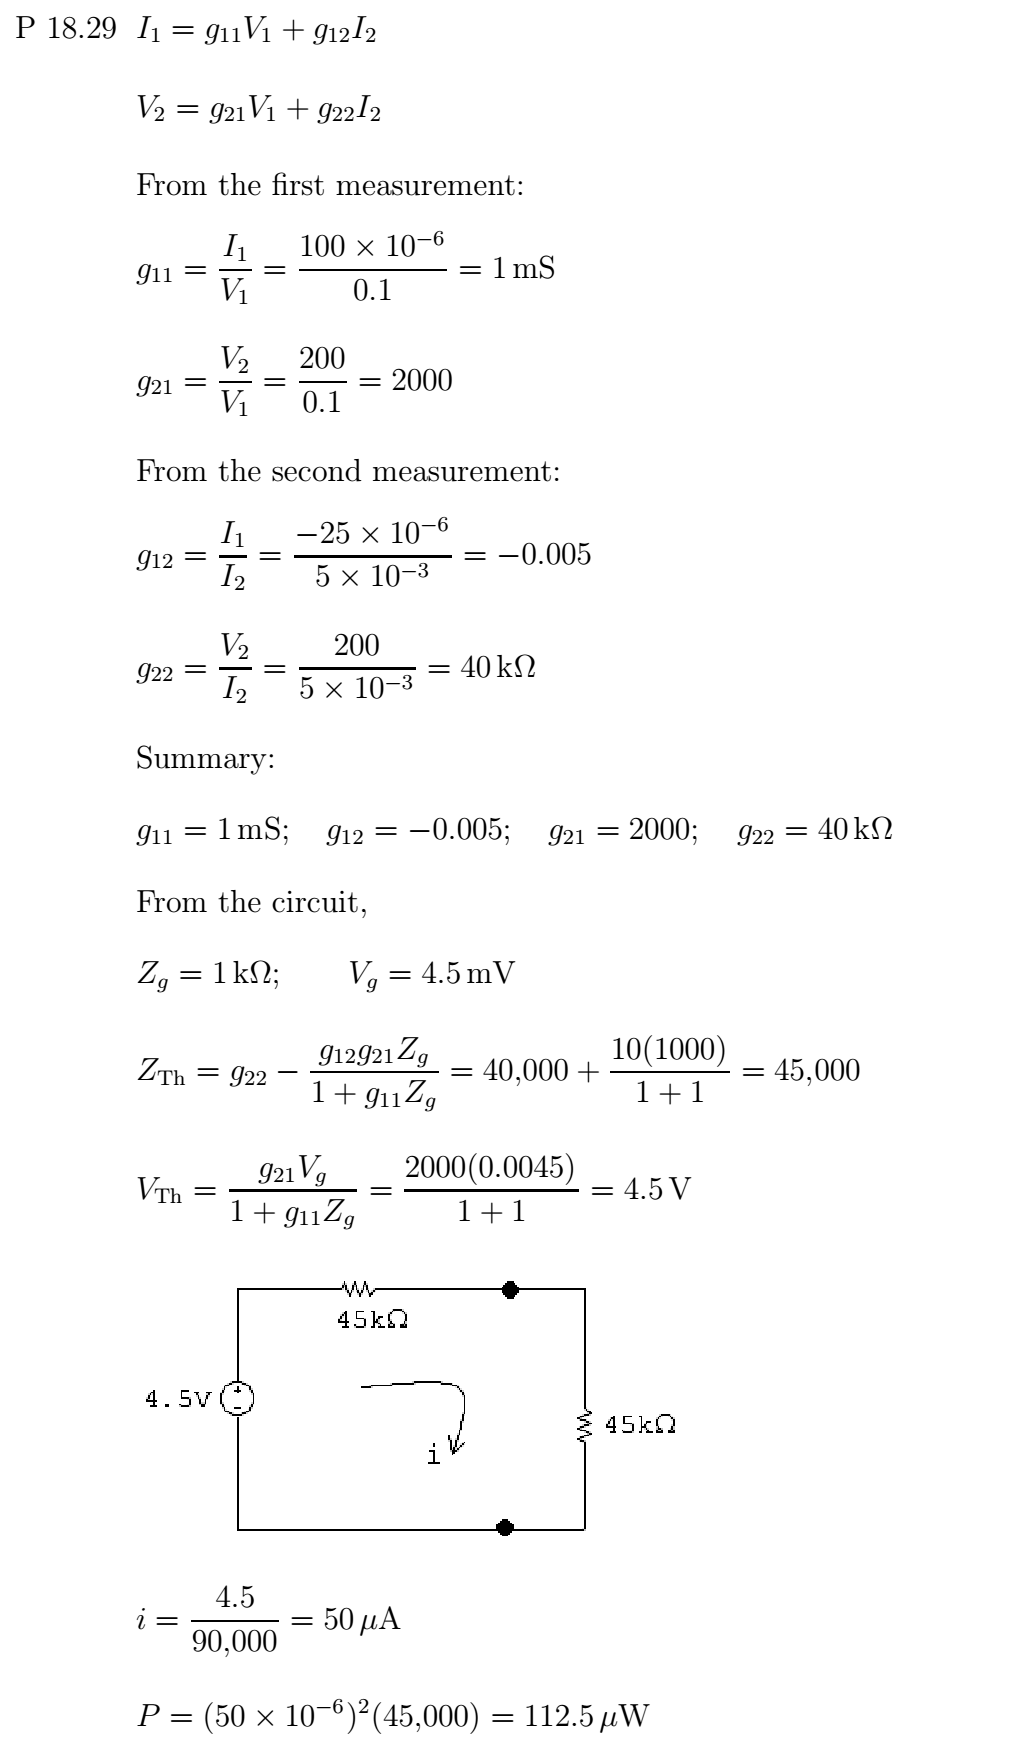
\includegraphics[width=\maxwidth{101.75614651279479em}]{image_11}
\end{flushleft}
\end{par}

\end{document}
